\documentclass[12pt,a4paper]{article}
\usepackage[utf8x]{inputenc}
\usepackage{ucs}
\usepackage{amsmath}
\usepackage{amsfonts}
\usepackage{amssymb}
\usepackage{graphicx}
\usepackage{grffile}
\usepackage{float}
\usepackage{multicol}
\usepackage[portuguese]{babel}
\title{MAT2456 - P2-2014}
\author{André Garnier Coutinho}
\setlength{\textwidth}{17cm}
\setlength{\textheight}{24cm}
\addtolength{\topmargin}{-2cm}
\addtolength{\oddsidemargin}{-2cm}

\newcommand{\re}{\mathbb{R}}

\newcommand{\sen}{\mbox{\,sen}}

\begin{document}
%%%%%%%%%%%%%%%%%%%%%%%%%%%%%%%%%%%%%%%%%%TURMA A%%%%%%%%%%%%%%%%%%%%%%%%%%%%%%%%%%%%%%%%%%%%%%%
\begin{center}
\textbf{Instituto de Matemática e Estatística da USP\\
MAT2455 - Cálculo Diferencial e Integral IV para Engenharia\\}
\textbf{2a. Prova - 2o. Semestre 2014 - 13/10/2014}
\end{center}

\noindent {\bf Turma A}

\noindent{\bf 1ª Questão:}
\begin{itemize}
	\item[a)] (1,0 ponto) Seja $ f(x) = \displaystyle\frac{1}{1+2x^3}$. Calcule $f^{(30)}(0)$.
	
	\item[b)] Obtenha uma expressão para a soma da série $\displaystyle\sum_{n=1}^\infty (-1)^n \, 2^n \, 9 n^2 \, x^{3n}$ 
	\item[c)] Encontre um valor para a soma do item $b)$, quando $x = \displaystyle\frac{1}{2}$.
\end{itemize}


\noindent{\bf \\ \\Solução:}
\begin{itemize}
    \item[a)] Sabe-se que $ \displaystyle\frac{1}{1-x} = \displaystyle\sum_{n=0}^\infty x^n $, para $|x|<1$ (soma da PG). Sendo assim:
    
    $$\frac{1}{1 + 2x^3} = \sum_{n=0}^\infty (-2 x^3), |-2x^3| < 1$$
    $$ = \sum_{n=0}^\infty (-1)^n  \, 2^n \, x^{3n}, |x| < \frac{1}{\sqrt[3]{2}} $$
    
    
    Sabe-se que para uma série de potencias positivas $ \, \displaystyle\sum_{k=0}^\infty a_k (x-x_0)^k $, $a_k$ é dado pelo coeficiênte de Taylor: $a_k = \displaystyle\frac{f^{(k)}(x_0)}{k!}$.
    
    Como a série encontrada foi expandida em torno de $x_0 = 0$, temos que: $a_{30} = \displaystyle\frac{f^{(30)}(0)}{30!}$, o qual é coeficiente de $x^{30}$. \\
    
    O termo geral da série obtida é dado por $ \bar{a}_n = (-1)^n  \, 2^n \, x^{3n}$.
    
    Para $n=10$, temos $\bar{a}_{10} = 2^{10} x^{30}$, o que significa que o coeficiente de $x^{30}$ na série é $2^{10}$.
    
    Sendo assim, temos: $ \displaystyle\frac{f^{(30)}(0)}{30!} = 2^{10} $
    
    $$ \therefore f^{(30)} = 2^{10} \, 30! $$


    \item[b)] Deseja-se encontrar uma expressão para $\displaystyle\sum_{n=1}^\infty (-1)^n \, 2^n \, 9 n^2 x^{3n}$.
    
     Pode-se observar que há uma certa semelhança entre os termos gerais desta série e da série do exercicio anterior. Repare que derivando em x, multiplicando por x, derivando mais uma vez e multplicando por x mais uma vez, chegamos na mesma expressão. Sendo assim:
     
     $$\frac{1}{1 + 2x^3} =  \sum_{n=0}^\infty (-1)^n  \, 2^n \, x^{3n}, |x| < \frac{1}{\sqrt[3]{2}} $$
     
     Derivando em x:
     
     $$\frac{-2 \cdot 3 x^2}{(1 + 2x^3)^2} =  \sum_{n=0}^\infty (-1)^n  \, 2^n \, 3 n \, x^{3n-1}, |x| < \frac{1}{\sqrt[3]{2}} $$
     
     $$ \Rightarrow \frac{-6 x^3}{(1 + 2x^3)^2} =  \sum_{n=0}^\infty (-1)^n  \, 2^n \, 3 n \, x^{3n}, |x| < \frac{1}{\sqrt[3]{2}} $$
     
     Derivando mais uma vez:
     
     $$ \frac{-6 [ (3 x^2) (1 + 2x^3)^2 - x^3 \cdot 2 (1 + 2 x^3) 6 x^2 ] }{(1 + 2x^3)^4} =  \sum_{n=0}^\infty (-1)^n  \, 2^n \, 9 n^2 \, x^{3n-1}, |x| < \frac{1}{\sqrt[3]{2}} $$
     
     $$ \frac{-6 [ 3 x^2 - 6 x^5 ] }{(1 + 2x^3)^3} =  \sum_{n=0}^\infty (-1)^n  \, 2^n \, 9 n^2 \, x^{3n-1}, |x| < \frac{1}{\sqrt[3]{2}} $$
     
     $$ \therefore \sum_{n=0}^\infty (-1)^n  \, 2^n \, 9 n^2 \, x^{3n} = \frac{-18 x^3 (1 - 2 x^3)}{(1 + 2 x^3)^3} , |x| < \frac{1}{\sqrt[3]{2}} $$
     
     \item[c)] Como $ x = \frac{1}{2}$ está dentro do intervalo de convergência da série do item $b)$, temos que:
     
     $$  \sum_{n=0}^\infty   \frac{(-1)^n  \, 9 n^2}{4^n} = \frac{-18 \cdot \frac{1}{8} (1 - 2 \cdot \frac{1}{8})}{(1 + 2  \cdot \frac{1}{8})^3} = -\frac{3^3 \, 4}{5^3} = -\frac{108}{125} $$
    

\end{itemize}
\ \

%---------------------------------------QUESTAO 2-----------------------------------------
\newpage

\noindent{\bf 2ª Questão:}

\begin{itemize}
\item[a)] (1,5 pontos) Seja $ f(x) = \begin{cases} \displaystyle\frac{e^{3x}-1}{x} \, , \, $ se $ x \neq 0 \\ 3 \, , \,\,\,\,\,\,\,\,\,\,\,\,\,\,\,\,\, $ se $x = 0 \end{cases} $

\begin{itemize}
\item[a1)] Encontre uma série numérica cuja soma seja igual a $ \displaystyle\int_0^{1/6} \, f(x) \, dx$.
\item[a2)] Encontre um valor aproximado para $ \displaystyle\int_0^{1/6} \, f(x) \, dx$, com erro, em módulo, menor que $10^{-4}$. 
\end{itemize}

\item[b)] (1,5 pontos) Sabendo que a série de Fourier de senos de $g(x) = x(\pi - x)$, em $[0, \pi]$ é

\begin{center}
$ \displaystyle\frac{8}{\pi} \Big( \sen x + \displaystyle\frac{\sen (3x)}{3^3} + \displaystyle\frac{\sen (5x)}{5^3} + ... \Big) \,$,
\end{center} 

calcule $ \displaystyle\sum_{n=0}^{\infty} \, \Big( \displaystyle\frac{1}{2n + 1} \Big)^6 $.

\end{itemize}

\noindent{\bf Solução:} \\

\begin{itemize}
\item[a1)] Sabe-se que:

$$ e^x  = \sum_{n=0}^\infty \frac{x^n}{n!} \, , \forall x \in \mathbb{R}$$

Sendo assim:

$$ e^{3x} - 1 = \sum_{n=0}^\infty \frac{(3x)^n}{n!} - 1 =  \sum_{n=1}^\infty \frac{3^n \, x^n}{n!} \, , \forall x \in \mathbb{R} $$
$$ \therefore \frac{e^{3x} - 1}{x} = \sum_{n=1}^\infty \frac{3^n \, x^{n-1}}{n!} \, , \forall x \neq 0 $$

Para x = 0:

$$ \sum_{n=1}^\infty \frac{3^n \, x^{n-1}}{n!} = 3 $$

$$ \therefore f(x) = \sum_{n=1}^\infty \frac{3^n \, x^{n-1}}{n!} \, , \forall x \in \mathbb{R} $$

Assim:

$$ \int_{0}^{x'} f(x) \, dx = \sum_{n=1}^\infty \frac{3^n \, x^{n}}{n \cdot n!} \Big|_{0}^{x'} = \sum_{n=1}^\infty \frac{3^n \, (x')^{n}}{n \cdot n!} \, , \forall x \in \mathbb{R} $$

Para $ x' = 1/6$:

$$ \int_{0}^{1/6} f(x) \, dx =  \sum_{n=1}^\infty \frac{3^n}{ 6^n \, n \cdot n!} = \sum_{n=1}^\infty \frac{1}{ 2^n \, n \cdot n!} $$

\item[a2)] Deseja-se calcular $ \displaystyle\int_{0}^{1/6} f(x) \, dx$ com $erro < \varepsilon = 10^{-4}$. Do item anterior, sabe-se que:

$$ \int_{0}^{1/6} f(x) \, dx = \sum_{n=1}^\infty \frac{1}{ 2^n \, n \cdot n!} \simeq \sum_{n=1}^k \frac{1}{ 2^n \, n \cdot n!}  $$

O erro da aproximação é dado por:

$$ erro = \sum_{n=k+1}^\infty \frac{1}{ 2^n \, n \cdot n!} $$

Rapare que se não tivessemos $ n \cdot n!$ multiplicando $2^n$, teríamos a soma de uma PG de razão $1/2$, a qual é fácil de calcular o valor exato da soma.

Repare também que o termo $ \frac{1}{n \cdot n!} $ é sempre decrescente, ou seja:

$$ \frac{1}{n \cdot n!} \leq \frac{1}{ (k+1) \cdot (k+1)!} ,\ \forall n \geq k+1 $$

Sendo assim:

$$ erro = \sum_{n=k+1}^\infty \frac{1}{ 2^n \, n \cdot n!} \leq \frac{1}{(k+1)(k+1)!} \sum_{n=k+1}^\infty \frac{1}{ 2^n} < \varepsilon $$

$$ \frac{1}{(k+1)(k+1)!} \frac{ \frac{1}{2^{k+1}} }{1 - \frac{1}{2}} = \frac{1}{(k+1)(k+1)!} \frac{1}{2^k} < \varepsilon  $$

$$ \therefore 2^k (k+1)(k+1)! > \frac{1}{\varepsilon} = 10^4 $$

Para $k = 5$:

$$ 2^k (k+1)(k+1)! = 32 \cdot 6 \cdot 720 = 192 \cdot 720 > 10^4 $$

Portanto: 

$$ \int_{0}^{1/6} f(x) \, dx  \simeq \sum_{n=1}^5 \frac{1}{ 2^n \, n \cdot n!}  $$

Com $erro < 10^{-4}$.

\item[b)] Seja $\tilde{g}(x)$ a extensão ímpar de $g(x)$. A série de Fourier de $\tilde{g}(x)$ é a série de senos de $g(x)$. Sabe-se que os coeficientes da série de Fourier de $\tilde{g}(x)$ são:

$$ a_0 = a_n = 0 $$
$$ b_{2n} = 0 $$
$$ b_{2n+1} = \frac{8}{\pi (2n + 1)^3} $$

Aplicando a identidade de Parceval:

$$ \frac{a_0}{2} + \sum_{n=1}^\infty \Big( a_n^2 + b_n^2 \Big) =\frac{1}{\pi} \int_{-\pi}^{\pi} \tilde{g}^2(x) \, dx $$

$$ \Rightarrow  \sum_{n=1}^\infty  b_{2n}^2 + \sum_{n=0}^\infty  b_{2n+1}^2  =\frac{1}{\pi} \int_{-\pi}^{\pi} \tilde{g}^2(x) \, dx $$

Como $\tilde{g}(x)$ é impar, $\tilde{g}^2(x)$ é par. Além disso, como $\tilde{g}(x)$ é extensão ímpar de $g(x)$, $\tilde{g}(x) = g(x)$ para $x \in [0, \pi]$. Assim, temos:

$$ \sum_{n=0}^\infty  \frac{64}{\pi^2 (2n + 1)^6}  =\frac{2}{\pi} \int_{0}^{\pi} g^2(x) \, dx $$.

$$ \int_{0}^{\pi} g^2(x) \, dx = \int_{0}^{\pi} x^2 \pi^2 - 2 \pi x^3 + x^4 \, dx = \Big( \frac{\pi^2 x^3}{3} - \frac{ 2\pi x^4 }{4} + \frac{x^5}{5}  \Big)_0^\pi = \frac{\pi^5}{30} $$

$$ \therefore \sum_{n=0}^\infty  \frac{1}{ (2n + 1)^6} = \frac{\pi^2}{64} \cdot \frac{2}{\pi} \cdot \frac{\pi^5}{30} = \frac{\pi^6}{960}  $$

\end{itemize}

%---------------------------------------QUESTAO 3-----------------------------------------

\newpage
\noindent{\bf 3ª Questão: }
\begin{itemize}
\item[a)] (2,0 pontos) Seja

\begin{center}
$ f(x) = \displaystyle\begin{cases} 0 \, , \,\,\,\,\,\,\, $ se $ x \in \Big[-\pi, -\frac{\pi}{2} \Big[ \,$ ou $x \in \Big]\frac{\pi}{2}, \pi \Big] \\\\ 2|x| \,,$ se $ x \in \Big[-\frac{\pi}{2}, \frac{\pi}{2} \Big] \end{cases}$
\end{center}

Encontre a série de Fourier de $f$.

\item[b)] (1,5 pontos) Se $S(x)$ é a soma da série encontrada em $a)$, esboce o gráfico de $S$ no intervalo $[-3\pi,3\pi]$, calcule $S\Big(39 \displaystyle\frac{\pi}{2}\Big)$ e $S\Big(1223 \displaystyle\frac{\pi}{8}\Big)$.

\end{itemize}


\noindent{\bf Solução:}
\\

\begin{itemize}
\item[a)]

$$ a_0 = \frac{1}{\pi} \int_{-\pi}^\pi f(x) \, dx = \frac{1}{\pi} \int_{-\frac{\pi}{2}}^{\frac{\pi}{2}} 2 |x| \, dx = \frac{2}{\pi} \int_{0}^{\frac{\pi}{2}} 2 x \, dx = \frac{2}{\pi} x^2 \Big|_0^{\frac{\pi}{2}} = \frac{\pi}{2} $$

$$ a_n = \frac{1}{\pi} \int_{-\pi}^\pi f(x) \cos (n x) \, dx = \frac{1}{\pi} \int_{-\frac{\pi}{2}}^{\frac{\pi}{2}} 2 |x| \cos (n x) \, dx = \frac{2}{\pi} \int_{0}^{\frac{\pi}{2}} 2 x \cos (n x) \, dx $$

$$ \int_{0}^{\frac{\pi}{2}}  x \cos (n x) \, dx =  \frac{x \sen (nx)}{n} \Big|_0^\frac{\pi}{2} -  \int_{0}^{\frac{\pi}{2}} \frac{\sen(nx)}{n} \,dx = \frac{\pi \sen( \frac{n \pi}{2})}{2 n} + \frac{\cos (nx)}{n^2} \Big|_0^\frac{\pi}{2}    $$

$$ = \frac{\pi \sen( \frac{n \pi}{2})}{2 n} + \frac{ ( \cos (\frac{n \pi}{2}) -1)}{n^2} $$

$$ \therefore a_n =  \frac{ 2 \sen( \frac{n \pi}{2})}{ n} +  \frac{ 4 ( \cos (\frac{n \pi}{2}) -1)}{\pi n^2} $$

\begin{center}
$b_n = \displaystyle\frac{1}{\pi} \displaystyle\int_{-\pi}^\pi f(x) \sen (n x) \, dx = 0 \,\,$ (função ímpar)
\end{center}

$$ \therefore S(x) = \frac{a_0}{2} + \sum_{n=1}^\infty \Big( a_n \cos(nx) + b_n \sen(nx) \Big) = \frac{\pi}{4} + \sum_{n=1}^\infty \Big( \frac{ 2 \sen( \frac{n \pi}{2})}{ n} +  \frac{ 4 ( \cos (\frac{n \pi}{2}) -1)}{\pi n^2} \Big) \cos (nx) $$

\item[b)] Pelo toerema da convergência da série de Fourier, $S(x)$ converge para:

\begin{itemize}
\item[•] Para $x \in  (-\pi,\pi)$:
	\begin{itemize}
	\item[-] $f(x), \,$ onde f(x) é contínua
	\item[-] A média dos limites laterais, onde f(x) é descontínua
	\end{itemize}
\item[•] $\displaystyle\frac{f(\pi)+f(-\pi)}{2}, \, $ para $ x = \pi $ ou $ x = -\pi $ 
\item[•] Para $x \notin [ -\pi,\pi]$: repete-se periodicamente.
\end{itemize}

\begin{figure}[H]
	\centering
	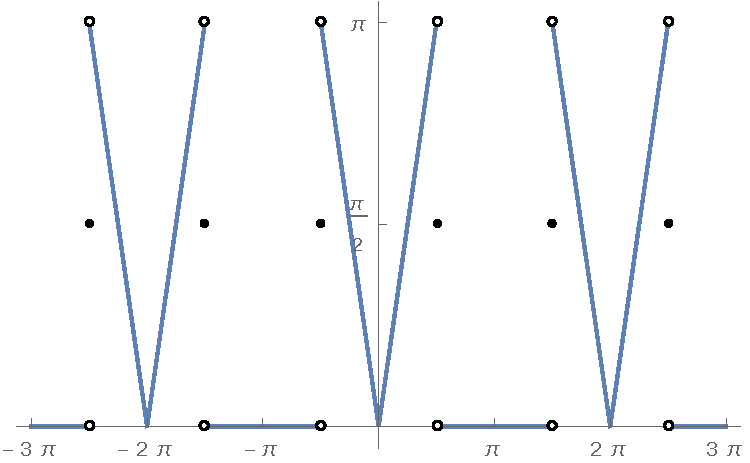
\includegraphics[scale=0.7]{Fourier.pdf}  
	\caption{Série de Fourier de $f(x)$ para $x \in [-3\pi, 3\pi]$}
	\label{fig:figura1}
\end{figure}

Sendo assim:
$$ S\Big(\frac{39 \pi}{2}\Big) = S\Big(17\pi + \frac{\pi}{2}\Big) = S\Big(\pi + \frac{\pi}{2}\Big) = S\Big(- \frac{\pi}{2}\Big) = \frac{1}{2} ( \lim_{x \rightarrow - \frac{\pi}{2}^+ } f(x) + \lim_{x \rightarrow - \frac{\pi}{2}^- } f(x) ) = \frac{1}{2} ( \pi + 0) = \frac{\pi}{2} $$

$$ S\Big(1223 \cdot \frac{\pi}{8}\Big) = S\Big(152\pi + \frac{7 \pi}{8}\Big) = S\Big(\frac{7\pi}{8}\Big) = f\Big(\frac{7\pi}{8}\Big) = 0 $$

\end{itemize}

\newpage
%%%%%%%%%%%%%%%%%%%%%%%%%%%%%%%%%%%%%%%%%%TURMA B%%%%%%%%%%%%%%%%%%%%%%%%%%%%%%%%%%%%%%%%%%%%%%%
\begin{center}
\textbf{Instituto de Matemática e Estatística da USP\\
MAT2455 - Cálculo Diferencial e Integral IV para Engenharia\\}
\textbf{2a. Prova - 2o. Semestre 2014 - 13/10/2014}
\end{center}

\noindent {\bf Turma B}

\noindent{\bf 1ª Questão:}
\begin{itemize}
	\item[a)] (1,0 ponto) Seja $ f(x) = \displaystyle\frac{1}{1+3x^4}$. Calcule $f^{(40)}(0)$.
	
	\item[b)] Obtenha uma expressão para a soma da série $\displaystyle\sum_{n=1}^\infty (-1)^n \, 3^n \, 16 n^2 \, x^{4n}$ 
	\item[c)] Encontre um valor para a soma do item $b)$, quando $x = \displaystyle\frac{1}{2}$.
\end{itemize}


\noindent{\bf \\ \\Solução:}
\begin{itemize}
    \item[a)] Sabe-se que $ \displaystyle\frac{1}{1-x} = \displaystyle\sum_{n=0}^\infty x^n $, para $|x|<1$ (soma da PG). Sendo assim:
    
    $$\frac{1}{1 + 3x^4} = \sum_{n=0}^\infty (-3 x^4), |-3x^4| < 1$$
    $$ = \sum_{n=0}^\infty (-1)^n  \, 3^n \, x^{4n}, |x| < \frac{1}{\sqrt[4]{3}} $$
    
    
    Sabe-se que para uma série de potencias positivas $ \, \displaystyle\sum_{k=0}^\infty a_k (x-x_0)^k $, $a_k$ é dado pelo coeficiênte de Taylor: $a_k = \displaystyle\frac{f^{(k)}(x_0)}{k!}$.
    
    Como a série encontrada foi expandida em torno de $x_0 = 0$, temos que: $a_{40} = \displaystyle\frac{f^{(40)}(0)}{40!}$, o qual é coeficiente de $x^{40}$. \\
    
    O termo geral da série obtida é dado por $ \bar{a}_n = (-1)^n  \, 3^n \, x^{4n}$.
    
    Para $n=10$, temos $\bar{a}_{10} = 3^{10} x^{40}$, o que significa que o coeficiente de $x^{40}$ na série é $3^{10}$.
    
    Sendo assim, temos: $ \displaystyle\frac{f^{(40)}(0)}{40!} = 3^{10} $
    
    $$ \therefore f^{(40)} = 3^{10} \, 40! $$


    \item[b)] Deseja-se encontrar uma expressão para $\displaystyle\sum_{n=1}^\infty (-1)^n \, 3^n \, 16 n^2 x^{4n}$.
    
     Pode-se observar que há uma certa semelhança entre os termos gerais desta série e da série do exercicio anterior. Repare que derivando em x, multiplicando por x, derivando mais uma vez e multplicando por x mais uma vez, chegamos na mesma expressão. Sendo assim:
     
     $$\frac{1}{1 + 3x^4} =  \sum_{n=0}^\infty (-1)^n  \, 3^n \, x^{4n}, |x| < \frac{1}{\sqrt[4]{3}} $$
     
     Derivando em x:
     
     $$\frac{-3 \cdot 4 x^3}{(1 + 3x^4)^2} =  \sum_{n=0}^\infty (-1)^n  \, 3^n \, 4 n \, x^{4n-1}, |x| < \frac{1}{\sqrt[4]{3}} $$
     
     $$ \Rightarrow \frac{-12 x^4}{(1 + 3x^4)^2} =  \sum_{n=0}^\infty (-1)^n  \, 3^n \, 4 n \, x^{4n}, |x| < \frac{1}{\sqrt[4]{3}} $$
     
     Derivando mais uma vez:
     
     $$ \frac{-12 [ (4 x^3) (1 + 3x^4)^2 - x^4 \cdot 2 (1 + 3 x^4) 12 x^3 ] }{(1 + 3x^4)^4} =  \sum_{n=0}^\infty (-1)^n  \, 3^n \, 16 n^2 \, x^{4n-1}, |x| < \frac{1}{\sqrt[4]{3}} $$
     
     $$ \frac{-12 [ 4 x^3 - 12 x^7 ] }{(1 + 3x^4)^3} =  \sum_{n=0}^\infty (-1)^n  \, 3^n \, 16 n^2 \, x^{4n-1}, |x| < \frac{1}{\sqrt[4]{3}} $$
     
     $$ \therefore \sum_{n=0}^\infty (-1)^n  \, 3^n \, 16 n^2 \, x^{4n} = \frac{-18 x^3 (1 - 2 x^3)}{(1 + 2 x^3)^3} , |x| < \frac{1}{\sqrt[4]{3}} $$
     
     \item[c)] Como $ x = \frac{1}{2}$ está dentro do intervalo de convergência da série do item $b)$, temos que:
     
     $$  \sum_{n=0}^\infty   \frac{(-1)^n  \, 9 n^2}{4^n} = \frac{-18 \cdot \frac{1}{8} (1 - 2 \cdot \frac{1}{8})}{(1 + 2  \cdot \frac{1}{8})^3} = -\frac{3^3 \, 4}{5^3} = -\frac{108}{125} $$
    

\end{itemize}
\ \

%---------------------------------------QUESTAO 2-----------------------------------------
\newpage

\noindent{\bf 2ª Questão:}

\begin{itemize}
\item[a)] (1,5 pontos) Seja $ f(x) = \begin{cases} \displaystyle\frac{e^{3x}-1}{x} \, , \, $ se $ x \neq 0 \\ 3 \, , \,\,\,\,\,\,\,\,\,\,\,\,\,\,\,\,\, $ se $x = 0 \end{cases} $

\begin{itemize}
\item[a1)] Encontre uma série numérica cuja soma seja igual a $ \displaystyle\int_0^{1/6} \, f(x) \, dx$.
\item[a2)] Encontre um valor aproximado para $ \displaystyle\int_0^{1/6} \, f(x) \, dx$, com erro, em módulo, menor que $10^{-4}$. 
\end{itemize}

\item[b)] (1,5 pontos) Sabendo que a série de Fourier de senos de $g(x) = x(\pi - x)$, em $[0, \pi]$ é

\begin{center}
$ \displaystyle\frac{8}{\pi} \Big( \sen x + \displaystyle\frac{\sen (3x)}{3^3} + \displaystyle\frac{\sen (5x)}{5^3} + ... \Big) \,$,
\end{center} 

calcule $ \displaystyle\sum_{n=0}^{\infty} \, \Big( \displaystyle\frac{1}{2n + 1} \Big)^6 $.

\end{itemize}

\noindent{\bf Solução:} \\

\begin{itemize}
\item[a1)] Sabe-se que:

$$ e^x  = \sum_{n=0}^\infty \frac{x^n}{n!} \, , \forall x \in \mathbb{R}$$

Sendo assim:

$$ e^{3x} - 1 = \sum_{n=0}^\infty \frac{(3x)^n}{n!} - 1 =  \sum_{n=1}^\infty \frac{3^n \, x^n}{n!} \, , \forall x \in \mathbb{R} $$
$$ \therefore \frac{e^{3x} - 1}{x} = \sum_{n=1}^\infty \frac{3^n \, x^{n-1}}{n!} \, , \forall x \neq 0 $$

Para x = 0:

$$ \sum_{n=1}^\infty \frac{3^n \, x^{n-1}}{n!} = 3 $$

$$ \therefore f(x) = \sum_{n=1}^\infty \frac{3^n \, x^{n-1}}{n!} \, , \forall x \in \mathbb{R} $$

Assim:

$$ \int_{0}^{x'} f(x) \, dx = \sum_{n=1}^\infty \frac{3^n \, x^{n}}{n \cdot n!} \Big|_{0}^{x'} = \sum_{n=1}^\infty \frac{3^n \, (x')^{n}}{n \cdot n!} \, , \forall x \in \mathbb{R} $$

Para $ x' = 1/6$:

$$ \int_{0}^{1/6} f(x) \, dx =  \sum_{n=1}^\infty \frac{3^n}{ 6^n \, n \cdot n!} = \sum_{n=1}^\infty \frac{1}{ 2^n \, n \cdot n!} $$

\item[a2)] Deseja-se calcular $ \displaystyle\int_{0}^{1/6} f(x) \, dx$ com $erro < \varepsilon = 10^{-4}$. Do item anterior, sabe-se que:

$$ \int_{0}^{1/6} f(x) \, dx = \sum_{n=1}^\infty \frac{1}{ 2^n \, n \cdot n!} \simeq \sum_{n=1}^k \frac{1}{ 2^n \, n \cdot n!}  $$

O erro da aproximação é dado por:

$$ erro = \sum_{n=k+1}^\infty \frac{1}{ 2^n \, n \cdot n!} $$

Rapare que se não tivessemos $ n \cdot n!$ multiplicando $2^n$, teríamos a soma de uma PG de razão $1/2$, a qual é fácil de calcular o valor exato da soma.

Repare também que o termo $ \frac{1}{n \cdot n!} $ é sempre decrescente, ou seja:

$$ \frac{1}{n \cdot n!} \leq \frac{1}{ (k+1) \cdot (k+1)!} ,\ \forall n \geq k+1 $$

Sendo assim:

$$ erro = \sum_{n=k+1}^\infty \frac{1}{ 2^n \, n \cdot n!} \leq \frac{1}{(k+1)(k+1)!} \sum_{n=k+1}^\infty \frac{1}{ 2^n} < \varepsilon $$

$$ \frac{1}{(k+1)(k+1)!} \frac{ \frac{1}{2^{k+1}} }{1 - \frac{1}{2}} = \frac{1}{(k+1)(k+1)!} \frac{1}{2^k} < \varepsilon  $$

$$ \therefore 2^k (k+1)(k+1)! > \frac{1}{\varepsilon} = 10^4 $$

Para $k = 5$:

$$ 2^k (k+1)(k+1)! = 32 \cdot 6 \cdot 720 = 192 \cdot 720 > 10^4 $$

Portanto: 

$$ \int_{0}^{1/6} f(x) \, dx  \simeq \sum_{n=1}^5 \frac{1}{ 2^n \, n \cdot n!}  $$

Com $erro < 10^{-4}$.

\item[b)] Seja $\tilde{g}(x)$ a extensão ímpar de $g(x)$. A série de Fourier de $\tilde{g}(x)$ é a série de senos de $g(x)$. Sabe-se que os coeficientes da série de Fourier de $\tilde{g}(x)$ são:

$$ a_0 = a_n = 0 $$
$$ b_{2n} = 0 $$
$$ b_{2n+1} = \frac{8}{\pi (2n + 1)^3} $$

Aplicando a identidade de Parceval:

$$ \frac{a_0}{2} + \sum_{n=1}^\infty \Big( a_n^2 + b_n^2 \Big) =\frac{1}{\pi} \int_{-\pi}^{\pi} \tilde{g}^2(x) \, dx $$

$$ \Rightarrow  \sum_{n=1}^\infty  b_{2n}^2 + \sum_{n=0}^\infty  b_{2n+1}^2  =\frac{1}{\pi} \int_{-\pi}^{\pi} \tilde{g}^2(x) \, dx $$

Como $\tilde{g}(x)$ é impar, $\tilde{g}^2(x)$ é par. Além disso, como $\tilde{g}(x)$ é extensão ímpar de $g(x)$, $\tilde{g}(x) = g(x)$ para $x \in [0, \pi]$. Assim, temos:

$$ \sum_{n=0}^\infty  \frac{64}{\pi^2 (2n + 1)^6}  =\frac{2}{\pi} \int_{0}^{\pi} g^2(x) \, dx $$.

$$ \int_{0}^{\pi} g^2(x) \, dx = \int_{0}^{\pi} x^2 \pi^2 - 2 \pi x^3 + x^4 \, dx = \Big( \frac{\pi^2 x^3}{3} - \frac{ 2\pi x^4 }{4} + \frac{x^5}{5}  \Big)_0^\pi = \frac{\pi^5}{30} $$

$$ \therefore \sum_{n=0}^\infty  \frac{1}{ (2n + 1)^6} = \frac{\pi^2}{64} \cdot \frac{2}{\pi} \cdot \frac{\pi^5}{30} = \frac{\pi^6}{960}  $$

\end{itemize}

%---------------------------------------QUESTAO 3-----------------------------------------

\newpage
\noindent{\bf 3ª Questão: }
\begin{itemize}
\item[a)] (2,0 pontos) Seja

\begin{center}
$ f(x) = \displaystyle\begin{cases} 0 \, , \,\,\,\,\,\,\, $ se $ x \in \Big[-\pi, -\frac{\pi}{2} \Big[ \,$ ou $x \in \Big]\frac{\pi}{2}, \pi \Big] \\\\ 2|x| \,,$ se $ x \in \Big[-\frac{\pi}{2}, \frac{\pi}{2} \Big] \end{cases}$
\end{center}

Encontre a série de Fourier de $f$.

\item[b)] (1,5 pontos) Se $S(x)$ é a soma da série encontrada em $a)$, esboce o gráfico de $S$ no intervalo $[-3\pi,3\pi]$, calcule $S\Big(39 \displaystyle\frac{\pi}{2}\Big)$ e $S\Big(1223 \displaystyle\frac{\pi}{8}\Big)$.

\end{itemize}


\noindent{\bf Solução:}
\\

\begin{itemize}
\item[a)]

$$ a_0 = \frac{1}{\pi} \int_{-\pi}^\pi f(x) \, dx = \frac{1}{\pi} \int_{-\frac{\pi}{2}}^{\frac{\pi}{2}} 2 |x| \, dx = \frac{2}{\pi} \int_{0}^{\frac{\pi}{2}} 2 x \, dx = \frac{2}{\pi} x^2 \Big|_0^{\frac{\pi}{2}} = \frac{\pi}{2} $$

$$ a_n = \frac{1}{\pi} \int_{-\pi}^\pi f(x) \cos (n x) \, dx = \frac{1}{\pi} \int_{-\frac{\pi}{2}}^{\frac{\pi}{2}} 2 |x| \cos (n x) \, dx = \frac{2}{\pi} \int_{0}^{\frac{\pi}{2}} 2 x \cos (n x) \, dx $$

$$ \int_{0}^{\frac{\pi}{2}}  x \cos (n x) \, dx =  \frac{x \sen (nx)}{n} \Big|_0^\frac{\pi}{2} -  \int_{0}^{\frac{\pi}{2}} \frac{\sen(nx)}{n} \,dx = \frac{\pi \sen( \frac{n \pi}{2})}{2 n} + \frac{\cos (nx)}{n^2} \Big|_0^\frac{\pi}{2}    $$

$$ = \frac{\pi \sen( \frac{n \pi}{2})}{2 n} + \frac{ ( \cos (\frac{n \pi}{2}) -1)}{n^2} $$

$$ \therefore a_n =  \frac{ 2 \sen( \frac{n \pi}{2})}{ n} +  \frac{ 4 ( \cos (\frac{n \pi}{2}) -1)}{\pi n^2} $$

\begin{center}
$b_n = \displaystyle\frac{1}{\pi} \displaystyle\int_{-\pi}^\pi f(x) \sen (n x) \, dx = 0 \,\,$ (função ímpar)
\end{center}

$$ \therefore S(x) = \frac{a_0}{2} + \sum_{n=1}^\infty \Big( a_n \cos(nx) + b_n \sen(nx) \Big) = \frac{\pi}{4} + \sum_{n=1}^\infty \Big( \frac{ 2 \sen( \frac{n \pi}{2})}{ n} +  \frac{ 4 ( \cos (\frac{n \pi}{2}) -1)}{\pi n^2} \Big) \cos (nx) $$

\item[b)] Pelo toerema da convergência da série de Fourier, $S(x)$ converge para:

\begin{itemize}
\item[•] Para $x \in  (-\pi,\pi)$:
	\begin{itemize}
	\item[-] $f(x), \,$ onde f(x) é contínua
	\item[-] A média dos limites laterais, onde f(x) é descontínua
	\end{itemize}
\item[•] $\displaystyle\frac{f(\pi)+f(-\pi)}{2}, \, $ para $ x = \pi $ ou $ x = -\pi $ 
\item[•] Para $x \notin [ -\pi,\pi]$: repete-se periodicamente.
\end{itemize}

\begin{figure}[H]
	\centering
	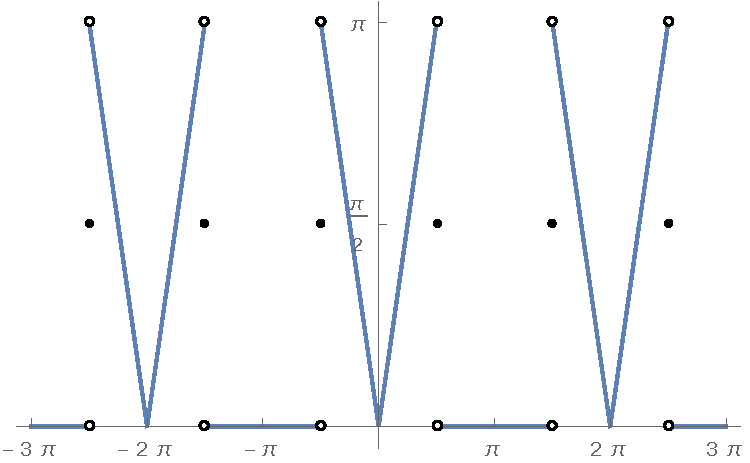
\includegraphics[scale=0.7]{Fourier.pdf}  
	\caption{Série de Fourier de $f(x)$ para $x \in [-3\pi, 3\pi]$}
	\label{fig:figura2}
\end{figure}

Sendo assim:
$$ S\Big(\frac{39 \pi}{2}\Big) = S\Big(17\pi + \frac{\pi}{2}\Big) = S\Big(\pi + \frac{\pi}{2}\Big) = S\Big(- \frac{\pi}{2}\Big) = \frac{1}{2} ( \lim_{x \rightarrow - \frac{\pi}{2}^+ } f(x) + \lim_{x \rightarrow - \frac{\pi}{2}^- } f(x) ) = \frac{1}{2} ( \pi + 0) = \frac{\pi}{2} $$

$$ S\Big(1223 \cdot \frac{\pi}{8}\Big) = S\Big(152\pi + \frac{7 \pi}{8}\Big) = S\Big(\frac{7\pi}{8}\Big) = f\Big(\frac{7\pi}{8}\Big) = 0 $$

\end{itemize}


\end{document} 
